\documentclass[aspectratio=1610]{beamer}
\usepackage[T1]{fontenc}
\usetheme{wildcat}
\usetikzlibrary{arrows.meta,angles,quotes,calc,intersections,positioning}

\usepackage{amsmath,amssymb,amsfonts}
\usepackage{booktabs}
\usepackage{relsize}
\usepackage{pgfplots}
\pgfplotsset{compat=1.16}
\usepackage{array}
\usepackage{siunitx}

\usepackage{jupyter}

\let\oldfootnotesize\footnotesize
\renewcommand*{\footnotesize}{\oldfootnotesize\tiny}

\def\mathdefault#1{#1}
\everymath=\expandafter{\the\everymath\displaystyle}


\title{Scattering Kinematics \\
       {\small\it NE 630 - Lecture 7}}

\date{\input{term.txt} \\ {\footnotesize Git SHA: \input{git_sha.txt}}}

\author{Jeremy Roberts}


\definecolor{ksupurple}{HTML}{512888}
\definecolor{orange}{HTML}{CA7C1B}

\begin{document}

\begin{frame}
\titlepage
\end{frame}
 
 
%%%%%%%%%%%%%%%%%%%%%%%%%%%%%%%%%%%%%%%%%%%%%%%%%%%
\begin{frame}{Primary Objective}

Students will be able to 

\vfill

\begin{quote}
\textcolor{wcprimary}{Estimate the number of elastic collisions a neutron of energy $E$ must make with a nucleus of mass number $A$ to slow to an energy $E'$.}
\end{quote}

\vfill 

\end{frame}

%%%%%%%%%%%%%%%%%%%%%%%%%%%%%%%%%%%%%%%%%%%%%%%%%%%%%%%%%%%%%%%%%%%%%%%%%%%%%%
\begin{frame}{Review}



\begin{figure}[h]
    \centering
    \resizebox{0.95\textwidth}{!}{\input{figures/U238_inelastic.pgf}}
\end{figure}

Do any of these interactions involve {\bf threshold} reactions?
\end{frame}

\begin{frame}{Neutron Elastic Scattering}

\begin{columns}[T,onlytextwidth]

\begin{column}{0.52\textwidth}
\centering

% --- Lab-frame diagram ---
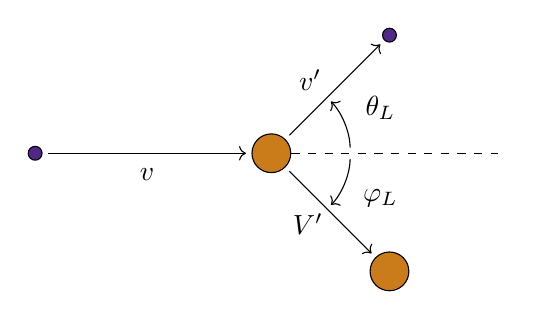
\begin{tikzpicture}[x=1.5cm,y=1.5cm]
  \node[circle,draw,fill=ksupurple,minimum size=5pt,inner sep=0pt] (a) at (-2,0) {};
  \node[circle,draw,fill=orange,minimum size=14pt,inner sep=0pt]   (b) at (0,0) {};
  \draw[->,shorten <=2pt,shorten >=2pt]
    (a) -- (b) node[midway,below=2pt] {$v$};
  \node[circle,draw,fill=ksupurple,minimum size=5pt,inner sep=0pt] (c) at (1,1) {};
  \node[circle,draw,fill=orange,minimum size=14pt,inner sep=0pt]   (d) at (1,-1) {};
  \node[] (e) at (2,0) {}; % dummy place holder
  \draw[->,shorten <=2pt,shorten >=2pt]
    (b) -- (c) node[pos=0.25,above=5pt] {$v'$};
  \draw[->,shorten <=2pt,shorten >=2pt]
    (b) -- (d) node[pos=0.25,below=5pt] {$V'$};
  \draw[-,dashed] (b) -- (e); % reference line
  \pic[draw,angle radius=10mm, ->, 
       angle eccentricity=1.5,"$\theta_{L}$",
       shorten <=2pt,shorten >=2pt] {angle = e--b--c};
  \pic[draw,angle radius=10mm, <-,
       angle eccentricity=1.5,"$\varphi_{L}$", 
       shorten <=2pt,shorten >=2pt] {angle = d--b--e};
\end{tikzpicture}

\vspace{0.8em}

% --- CM-frame diagram ---
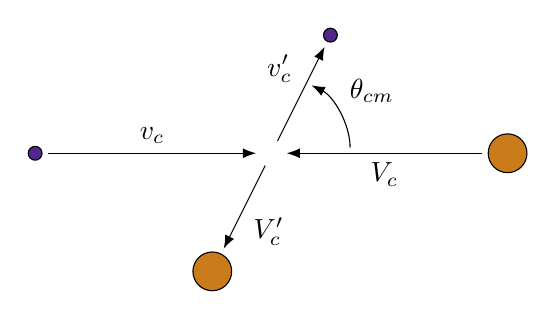
\begin{tikzpicture}[x=1.5cm,y=1.5cm,>=Latex]
  \node[circle,draw,fill=ksupurple,minimum size=5pt,inner sep=0pt] (a) at (-2,0) {};
  \node[circle,draw,fill=orange,minimum size=14pt,inner sep=0pt]   (b) at (2,0) {};
  \node[] (cm) at (0,0) {};
  \draw[->,shorten <=2pt,shorten >=2pt] (a) -- (cm) node[midway,above] {$v_c$};
  \draw[->,shorten <=2pt,shorten >=2pt] (b) -- (cm) node[midway,below] {$V_c$};
  \node[circle,draw,fill=ksupurple,minimum size=5pt,inner sep=0pt] (c) at (0.5,1) {};
  \draw[->,shorten <=1pt,shorten >=2pt] (cm) -- (c) node[midway,above left] {$v_c'$};
  \node[circle,draw,fill=orange,minimum size=14pt,inner sep=0pt] (d) at (-0.5,-1) {};
  \draw[->, shorten <=1pt,shorten >=2pt] (cm) -- (d) node[midway,below right] {$V_c'$};
  \pic[draw,angle radius=10mm, ->,
       angle eccentricity=1.5,"$\theta_{cm}$", 
       shorten <=2pt,shorten >=2pt] {angle = b--cm--c};
\end{tikzpicture}
\end{column}

\begin{column}{0.48\textwidth}
 
{\footnotesize
Conservation of momentum and energy in the {\bf laboratory} frame requires
\begin{align*}
m_n \,\mathbf{v} &= m_n \,\mathbf{v}' + M_N \,\mathbf{V}', \\
\tfrac{1}{2}m_n v^2 &= \tfrac{1}{2}m_n v'^2 + \tfrac{1}{2}M_N V'^2  \, .
\end{align*}
Similarly, in the {\bf center-of-mass} (CM) frame, we require
\begin{align*}
m_n \,\mathbf{v}_c + M_N \,\mathbf{V}_c &= \mathbf{0},\\
m_n \,\mathbf{v}_c' + M_N \,\mathbf{V}_c' &= \mathbf{0},\\
\tfrac{1}{2}m_n v_c^2 + \tfrac{1}{2}M_N V_c^2
&= \tfrac{1}{2}m_n v_c'^2 + \tfrac{1}{2}M_N V_c'^2.
\end{align*}
Elastic scattering (in the CM) frame requires
\begin{align*}
v_c' &= v_c \qquad \text{and} \qquad V_c' = V_c \, .
\end{align*}
Then, by defining
\begin{align*}
\mathbf{V}_{\rm CM} &= \frac{m_n}{m_n+M_N}\,\mathbf{v}
= \frac{1}{1+A}\,\mathbf{v} \, ,
\end{align*}
we can link the system quantities via 
\begin{align*}
\mathbf{v}' &= \mathbf{v}_c' + \mathbf{V}_{\rm CM} \qquad \text{and} \qquad
\mathbf{V}' = \mathbf{V}_c' + \mathbf{V}_{\rm CM} \, .
\end{align*}
Finally, vector properties (e.g., $\mathbf{x}\cdot \mathbf{y}=xy\cos(\theta)$)
can be used to define one-to-one relationships between $E'$ and $\theta_{cm}$
and between $\theta_L$ and $\theta_{cm}$.
See the Appendix for derivations.

}
\end{column}

\end{columns}
\end{frame}


%%%%%%%%%%%%%%%%%%%%%%%%%%%%%%%%%%%%%%%%%%%%%%%%%%%%%%%%%%%%%%%%%%%%%%%%%%%%%%
\begin{frame}{A Summary of Neutron Elastic Scattering Equations}
 
The outgoing energy \(E'\) and scattering angle
\(\theta_{cm}\) share a 1-to-1 relationship: \[
\frac{E'}{E} = \frac{A^2 + 2A\cos{\theta_{cm}} + 1}{(A+1)^2} \, .
\tag{Rydin 2.18}
\]

The scattering angles \(\theta_L\) and
\(\theta_{cm}\) also share a 1-to-1 relationship:

\[
  \cos \theta_L = \frac{1+A\cos\theta_{cm}} {\sqrt{A^2 + 2A \cos \theta_{cm} + 1}} \, .
  \tag{Rydin 2.21}
\]

For {\bf isotropic scattering} in the CM system, the ``average'' cosine of
\(\theta_L\) is \[
   \overline{\cos{\theta}_L} \equiv \bar{\mu} = \frac{2}{3A} 
   \tag{Rydin 2.56}
\]

{\bf Ponderables}: What values can $E'$ be?  $\cos \theta_{cm}$?  $\cos \theta_L$?
What happens to $\bar{\mu}$ as $A$ grows?

\end{frame}



%%%%%%%%%%%%%%%%%%%%%%%%%%%%%%%%%%%%%%%%%%%%%%%%%%%%%%%%%%%%%%%%%%%%%%%%%%%%%%
\begin{frame}{First, a Quick Summary of Probabilities}

If \(p(x)\) is a {\bf probability density function}, and if \(x\) is
restricted to a range of values called the {\bf support}, e.g.,
\(x_L \leq x \leq x_R\), then

\[
  \int^{x_U}_{x_L} p(x) dx = 1 \qquad \text{and} \qquad p(x) \leq 0 \, \text{for all}~x \in [x_U, x_L] \, .
\]

The {\bf probability} that \(x \in [a, b]\) (with \(a \geq x_L\) an
\(b \leq x_U\)) is

\[
 P(a \leq x \leq b) = \int^{b}_{a} p(x) dx \, .
\]

The {\bf expected value} (or ``average'') of some function \(f(x)\) is

\[
  E[f(x)] = \bar{f} =  \int^{x_U}_{x_L} f(x) p(x) dx \, .
\]


\end{frame}

%%%%%%%%%%%%%%%%%%%%%%%%%%%%%%%%%%%%%%%%%%%%%%%%%%%%%%%%%%%%%%%%%%%%%%%%%%%%%%
\begin{frame}{Transforming Probabilities}

Probability densities can be transformed from one variable to another.
For clarity, if $x$ and $y$ are random variable, we'll denote 
their densities by $p_X(x)$ and $p_Y(y)$.

\vfill 

Now, given $p_X(x)$, suppose that $y = f(x)$ is 
a one-to-one mapping. Then $p_X(x)dx = p_Y(y)dy$ and
\begin{equation*}
 p_Y(y) = \left | \frac{dx}{dy} \right | p_X(x) = \left | \frac{dy}{dx} \right |^{-1} p_X(x) \, .
\end{equation*}

\vfill

As a super simple example, let $x$ be uniform over $x \in [0, 1]$, and let $y = 2x-1$.  
Because $p_X(x) = 1$ for $x\in [0, 1]$ (and zero elsewhere), we have 
$p_Y(y) = |dx/dy|p_X(x) = 1/2$ for $y\in [-1, 1]$.
\end{frame}

%%%%%%%%%%%%%%%%%%%%%%%%%%%%%%%%%%%%%%%%%%%%%%%%%%%%%%%%%%%%%%%%%%%%%%%%%%%%%%
\begin{frame}{Energy Loss from Collisions}

The probability that a neutron of energy \(E\) strikes a nucleus of mass
\(A\) elastically and leaves with an energy \(E'\) is

\[
p(E\to E') = 
  \begin{cases}
    \frac{1}{(1-\alpha)E} & \alpha E \leq E' \leq E \\
    0 & \text{otherwise} \, ,
  \end{cases}
\tag{FNRP 2.47}
\]

where

\[
 \alpha = \frac{(A-1)^2}{(A+1)^2} \, .
 \tag{FRNP 2.48}
\]


% The notation \(p(E\to E')\) is common to particle transport, reactor
% physics, and related areas. A more common notation would be
% \(p(E'; E)\), which indicates that the (random) variable of interest is
% \(E'\), while \(E\) is a parameter. A familiar example is the Gaussian
% or normal distribution, often denoted by \(N(x; \mu, \sigma^2)\), where
% \(x\) is the variable, and the mean \(\mu\) and variance \(\sigma^2\) are
% parameters.

\pause 


{\bf Example}:  What is the expected outgoing energy $\bar{E}'$ of a neutron 
of energy $E$ after elastically colliding with a target of mass $A$?

\pause 
 
{\it\footnotesize Ans. $\bar{E}' = \frac{1}{2}(1+\alpha)E$}


\end{frame}


%%%%%%%%%%%%%%%%%%%%%%%%%%%%%%%%%%%%%%%%%%%%%%%%%%%%%%%%%%%%%%%%%%%%%%%%%%%%%%
\begin{frame}[fragile]{Slowing-Down Decrement}

The {\bf average logarithmic energy loss} aka {\bf slowing down
decrement} is

\[
  \xi = \overline{\ln(E/E')} 
    = 1 + \frac{\alpha}{1-\alpha}\ln\alpha 
  \tag{FNRP 2.54 and 2.56}
\]

The number of elastic collisions \(n\) needed to reduce a neutron's
energy from \(E_0\) to \(E_n\) is approximately

\[
  n = \frac{1}{\xi} \ln(E_0/E_n) \, .
  \tag{FNRP 2.59}
\]


\pause 


{\bf Example}:  How many collisions are required on the average to 
slow a 2 MeV neutron to 1 eV in water?

\pause 
 
{\it\footnotesize Ans. For water, $\xi = 0.93$, so $n = 0.93^{-1}\ln(2\cdot 10^6)\approx 16$.} 

\end{frame}
 
\begin{frame}[allowframebreaks]{Appendix: Derivation of Kinematics Equations}
 
\textbf{Set-up.} Target initially at rest in the lab; take $\hat{\mathbf{x}}$ along the incident neutron velocity $\mathbf{v}=v\,\hat{\mathbf{x}}$.
Let $m_n$ be the neutron mass and $M_N=A\,m_n$ the target mass. The CM speed is
\[
\mathbf{V}_{\rm CM}=\frac{m_n}{m_n+M_N}\,\mathbf{v}=\frac{1}{1+A}\,\mathbf{v},
\qquad 
v_c=\|\mathbf{v}-\mathbf{V}_{\rm CM}\|=\frac{A}{1+A}\,v.
\]
In the CM, elastic scattering preserves speeds and merely rotates directions, so
\(
\mathbf{v}_c' = v_c(\cos\theta_{cm}\,\hat{\mathbf{x}}+\sin\theta_{cm}\,\hat{\mathbf{y}})
\)
and the lab velocity is 
\(
\mathbf{v}'=\mathbf{v}_c'+\mathbf{V}_{\rm CM}.
\)
Below, write $\mu\equiv\cos\theta_{cm}$.

\medskip
\textbf{1) Energy–angle link \((E'/E\) vs.\ \(\theta_{cm})\).}
\[
\frac{E'}{E}=\frac{v'^2}{v^2}
=\frac{\|\mathbf{v}_c'+\mathbf{V}_{\rm CM}\|^2}{v^2}
=\frac{v_c^2+V_{\rm CM}^2+2v_cV_{\rm CM}\mu}{v^2}.
\]
Insert \(v_c=\tfrac{A}{1+A}v\) and \(V_{\rm CM}=\tfrac{1}{1+A}v\) to get
\[
\boxed{\;\displaystyle \frac{E'}{E}=\frac{A^2+2A\cos\theta_{cm}+1}{(A+1)^2}\;}
\tag{Rydin 2.18}
\]

\medskip
\textbf{2) Lab–CM angle link \((\theta_L\) vs.\ \(\theta_{cm})\).}
The lab scattering cosine is
\[
\cos\theta_L=\frac{\mathbf{v}'\!\cdot\!\hat{\mathbf{x}}}{\|\mathbf{v}'\|}
=\frac{v_c\cos\theta_{cm}+V_{\rm CM}}{v'}.
\]
Divide numerator and denominator by \(v\) and use
\(
v'/v=\sqrt{E'/E}
=\frac{\sqrt{A^2+2A\cos\theta_{cm}+1}}{A+1}
\)
(from part 1), to obtain
\[
\boxed{\;\displaystyle 
\cos\theta_L=\frac{1+A\cos\theta_{cm}}{\sqrt{A^2+2A\cos\theta_{cm}+1}}\;}
\tag{Rydin 2.21}
\]

\medskip
\textbf{3) Isotropic-in-CM average \(\overline{\cos\theta_L}\).}
For isotropic CM scattering, \(\mu=\cos\theta_{cm}\) is uniform on \([-1,1]\), so
\[
\overline{\cos\theta_L}=\frac{1}{2}\!\int_{-1}^{1}\!
\frac{1+A\mu}{\sqrt{A^2+2A\mu+1}}\,d\mu.
\]
Let \(u=\sqrt{A^2+2A\mu+1}\Rightarrow d\mu=(u/A)\,du\) and
\(1+A\mu=\tfrac{1}{2}(u^2-(A^2-1))\).
For nuclei \(A\ge 1\), the limits are \(u|_{\mu=-1}=A-1\) and \(u|_{\mu=1}=A+1\).
Thus
\begin{align*}
\overline{\cos\theta_L}
&=\frac{1}{2}\cdot\frac{1}{2A}\!\int_{A-1}^{A+1}\!\!\big(u^2-(A^2-1)\big)\,du\\
&=\frac{1}{4A}\Big[\tfrac{u^3}{3}-(A^2-1)u\Big]_{A-1}^{A+1}
=\boxed{\;\displaystyle \frac{2}{3A}\;} \, .
\tag{Rydin 2.56}
\end{align*}


\end{frame}

\end{document}

